\documentclass{beamer}

    % INFO
    \title[TADPOLE]{The Alzheimer’s Disease Prediction Of Longitudinal Evolution}
    \author{Kai Nichols}
    \institute[CSM]{Colorado School of Mines}
    \date{10/12/2018}

    % Add your macros
    \input{macros}

    % PACKAGES
    \usepackage{fontspec}
    \usepackage{graphicx}
    \usepackage{setspace}
    \usepackage{tikz}
    % \usepackage{customtitleslide}
    \usepackage{booktabs} % book-quality tables
    \usepackage[ruled,vlined]{algorithm2e}

    % FUNCTIONS
    \AtBeginSection[]
    {
        \begin{frame}<beamer>
        \tableofcontents[currentsection]
        \end{frame}
    }

    % \AtBeginSubsection[]
    % {
    %     \begin{frame}<beamer>
    %     \tableofcontents[currentsubsection]
    %     \end{frame}
    % }

    % THEMING
    \usetheme{Madrid}
    \usecolortheme{mines}

\begin{document}

    % Immersive Title Slide
    {
        \usebackgroundtemplate{\scalebox{-1}[1]{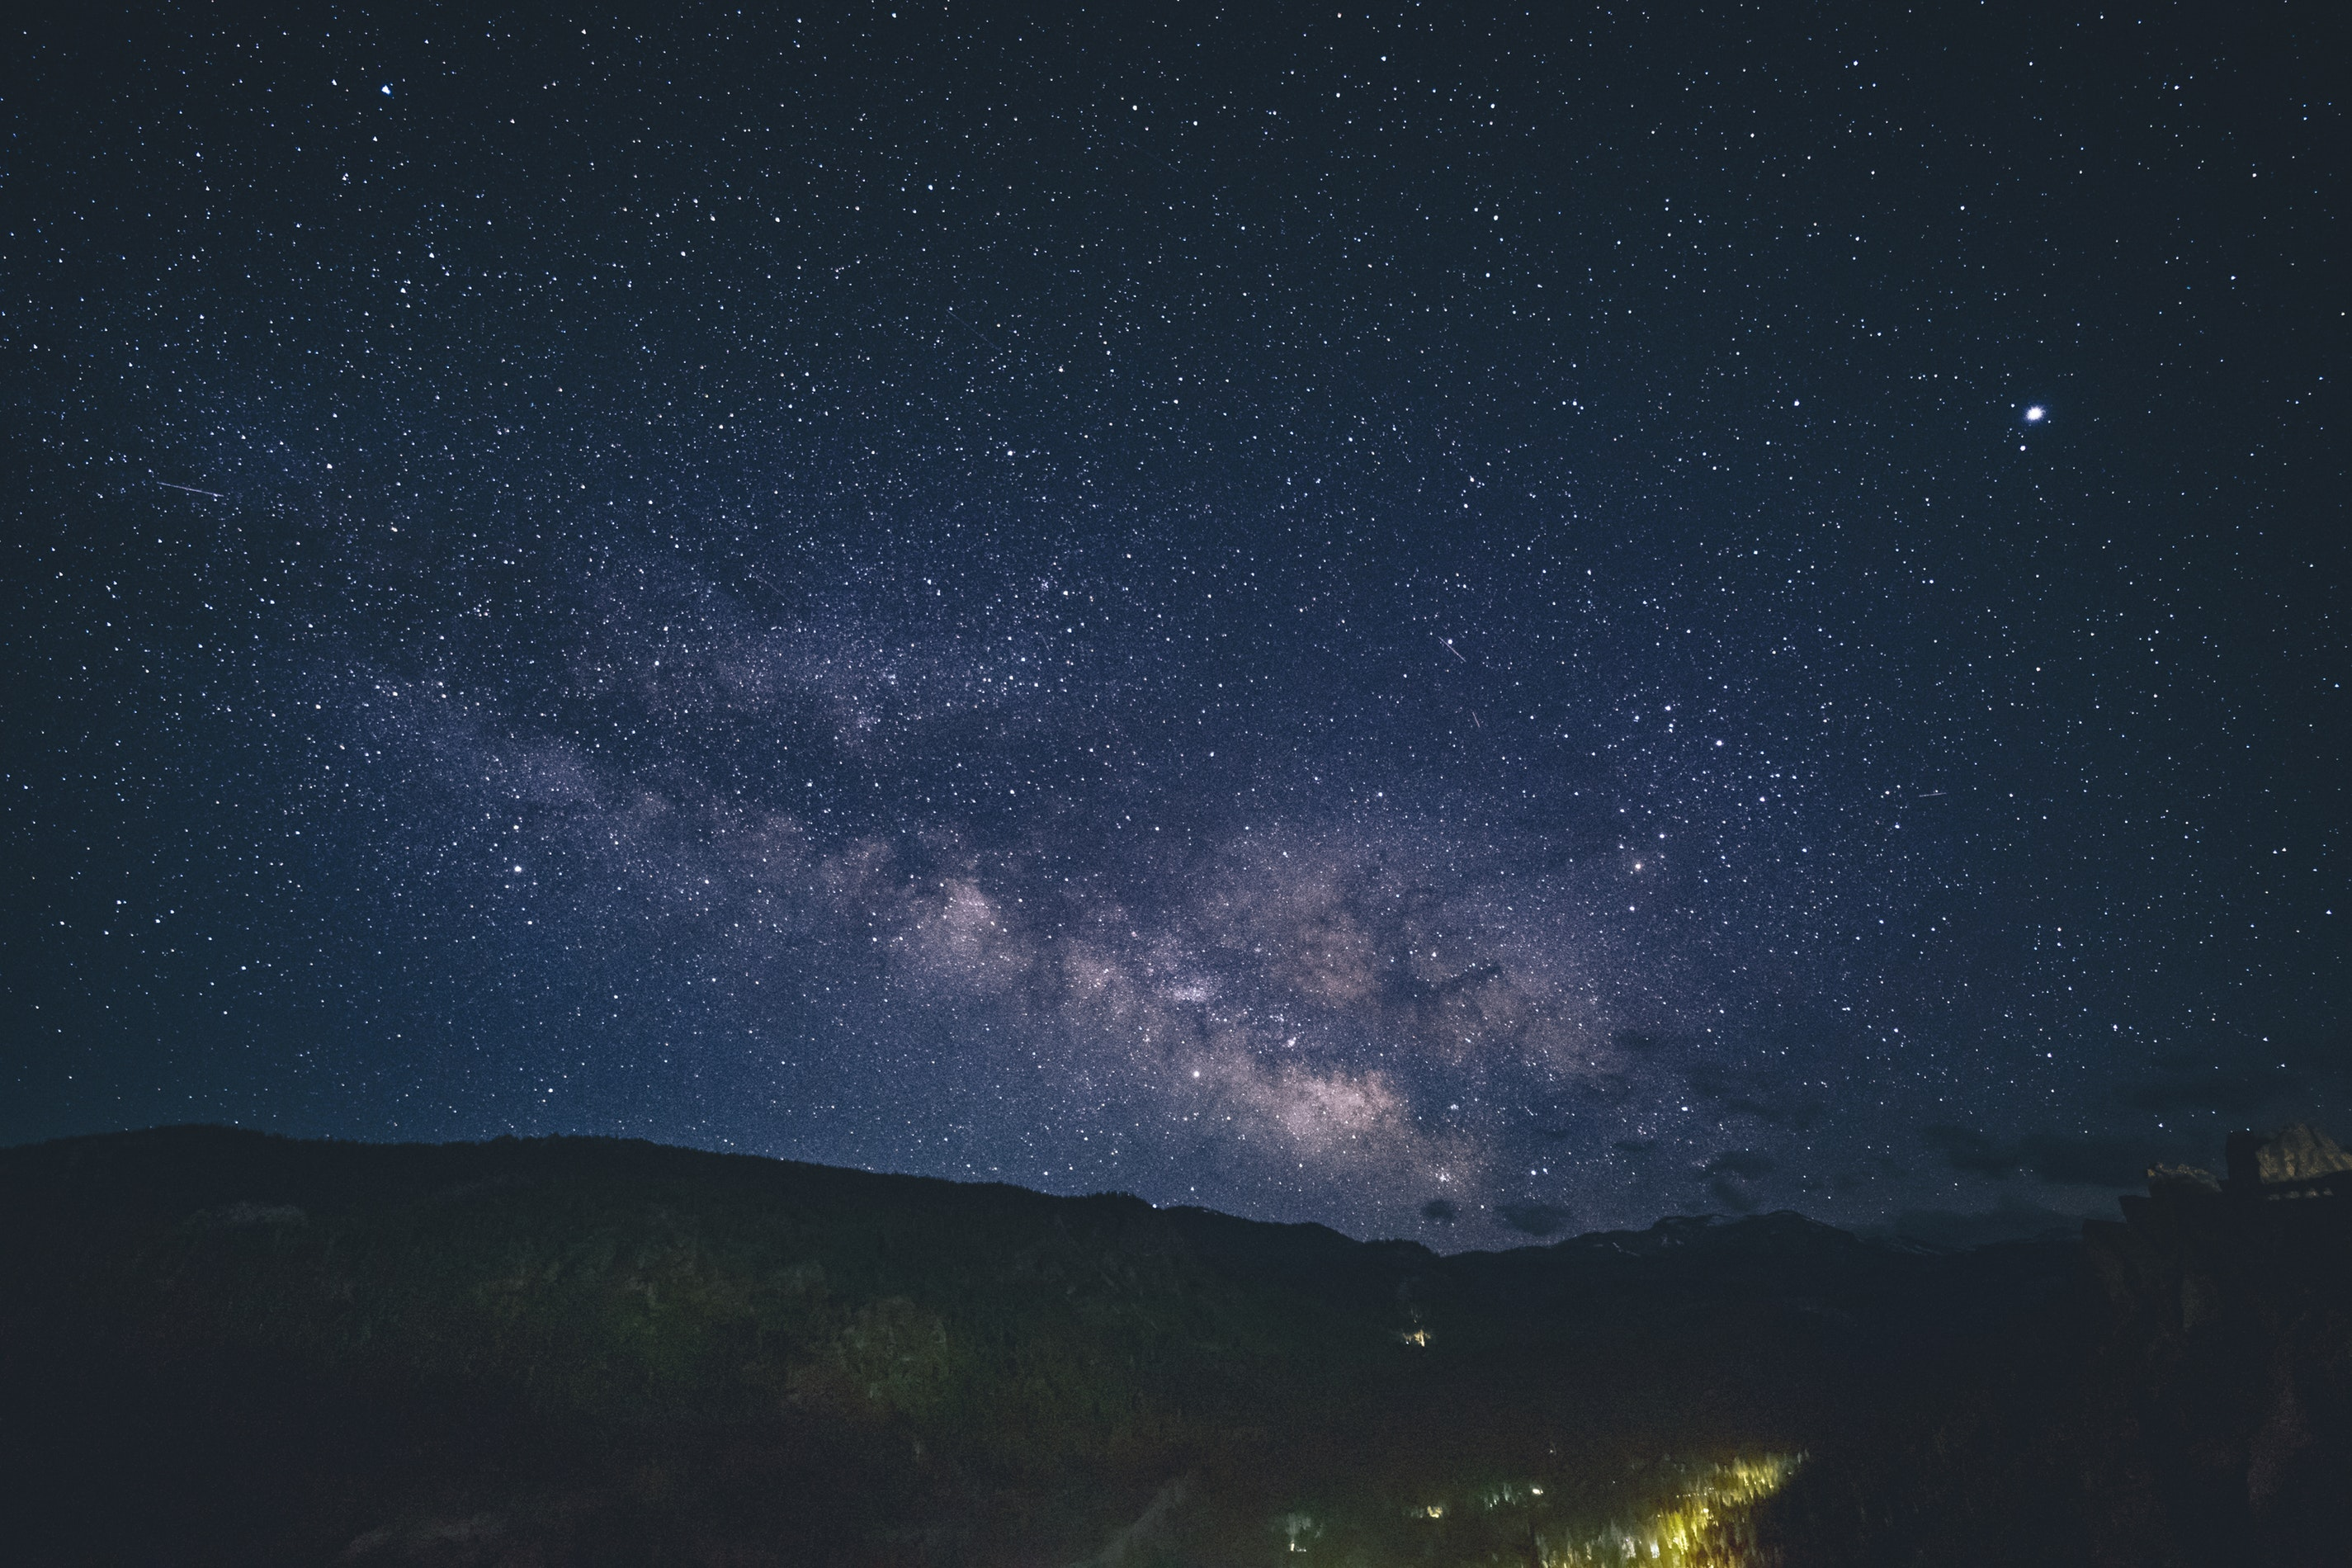
\includegraphics[width=\paperwidth, height=\paperheight]{images/background.jpeg}}}
        \begin{frame}[plain]
            \color{white}
            \vspace{4.8cm}
            {\Large \fontspec{Montserrat Bold} The Alzheimer’s Disease Prediction Of Longitudinal Evolution} \\
            \vspace{-0.2cm}
            {\color{white} \rule{\linewidth}{0.1mm}}
            \color{mineslightblue}
            {\Large \fontspec{Montserrat Regular} Kai Nichols}
            % Optional Advisor Section
            % \begin{spacing}{1.3}
            % {\Large \fontspec{Montserrat Light} Advised by} {\Large \fontspec{Montserrat Regular} Dr. Hua Wang}
            % \end{spacing}
            \begin{tikzpicture}[remember picture,overlay]
                \node[xshift=-0.5in,yshift=-0.4in, opacity=0.5] at (current page.north east) {
\includegraphics[width=0.2\textwidth]{images/logoWhite.png}};
            \end{tikzpicture}
        \end{frame}
    }

    \begin{frame}
        \frametitle{Contents}
        \begin{enumerate}
            \item TADPOLE Overview
            \item Modalities Available
            \item Data Access
        \end{enumerate}
    \end{frame}

    \begin{frame}
        \frametitle{TADPOLE Overview}
        The Alzheimer’s Disease Prediction Of Longitudinal Evolution (TADPOLE) is a dataset created and formatted by EuroPOND consortium with funding from the European Union’s Horizon 2020 research and innovation programme for use in a scientific challenge for senior high school students to develop machine learning algorithms to predict future evolution of individuals at risk of Alzheimer's Disease.\\
        \begin{center}
        
\includegraphics[height=.15\paperheight]{images/europond.png}
\includegraphics[height=.15\paperheight]{images/adni.png}
        \end{center}
    \end{frame}

    \begin{frame}
        \frametitle{TADPOLE Overview}
        \begin{columns}
        \begin{column}{0.5\textwidth}
            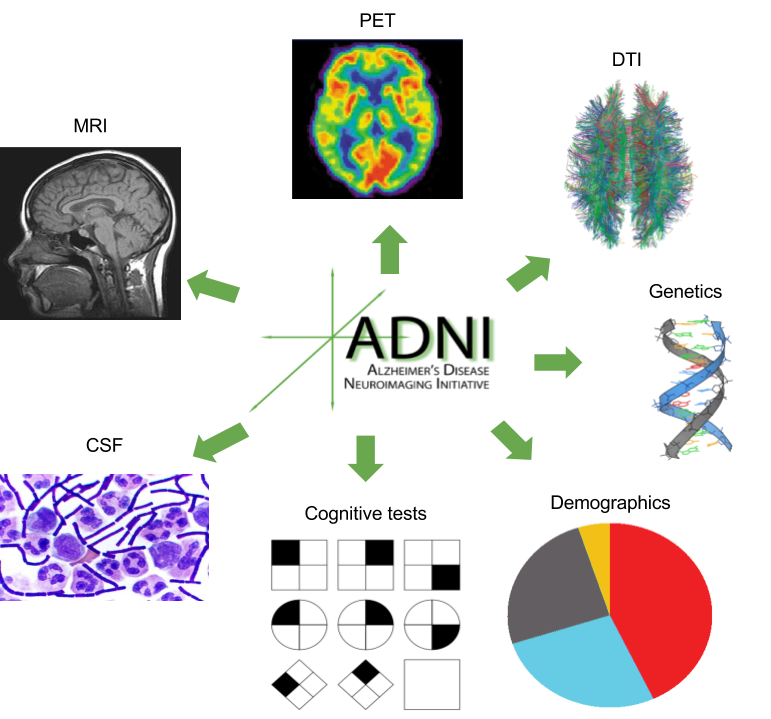
\includegraphics[width=\textwidth]{images/tadpoleoverview.png}
            \\
            Diagram showing TADPOLE biomarkers. Source of individual images: Wikimedia Commons
        \end{column}
        \begin{column}{0.5\textwidth}
            TADPOLE is a longitudinal data derived from the ADNI dataset with
            \begin{itemize}
                \item preselected features
                \item fairly preprocessed
                \item well documented data descriptions at the \href{https://tadpole.grand-challenge.org/}{tadpole website}
            \end{itemize}
        \end{column}
        \end{columns}
    \end{frame}

    \begin{frame}
        \frametitle{Modalities Overview}
        \begin{itemize}
            \item Diagnosis
            \item Demographics
            \item Cognitive Tests
            \item Genetic information
            \item MRI ROI
            \item PET ROI
        \end{itemize}
    \end{frame}

    \begin{frame}
        \frametitle{Diagnosis}
        Longitudinal \hfill 1730/1737 Patients (99.6\%)\\
        \vspace{0.2in}
        The entries specify both the current diagnosis and the baseline so, for example "MCI to Dementia" means that the current diagnosis is Dementia, while the diagnosis at the previous visit was MCI. EMCI,LMCI,SMC are only avaliable at the baseline.
        \begin{table}[]
        \begin{tabular}{ll}
        \hline
        Code                       & Meaning                                              \\ \hline
        \multicolumn{1}{|l|}{CN}   & \multicolumn{1}{l|}{Normal Aging/Cogntively Normal}  \\ \hline
        \multicolumn{1}{|l|}{EMCI/MCI} & \multicolumn{1}{l|}{Early Mild Cognitive Impairment} \\ \hline
        \multicolumn{1}{|l|}{LMCI} & \multicolumn{1}{l|}{Late Mild Cognitive Impairment}  \\ \hline
        \multicolumn{1}{|l|}{SMC}   & \multicolumn{1}{l|}{Significant Memory Concern}     \\ \hline
        \multicolumn{1}{|l|}{AD}   & \multicolumn{1}{l|}{Alzheimer’s disease}             \\ \hline
        \end{tabular}
        \end{table}
    \end{frame}

    \begin{frame}
        \frametitle{Demographics and Genetic}
        Demographics Static \hfill 1737/1737 Patients (100\%)\\
        \vspace{0.2in}

        \begin{columns}
        \begin{column}{0.5\textwidth}
            \begin{itemize}
                \item Age
                \item Sex
                \item Education
            \end{itemize}
        \end{column}
        \begin{column}{0.5\textwidth}
            \begin{itemize}
                \item Ethnicity
                \item Race
                \item Marital Status
            \end{itemize}
        \end{column}
        \end{columns}
        \vspace{0.2in}
        Genetic (ApoE4)
        Static \hfill 1725/1737 Patients (99.3\%)
        \begin{itemize}
            \item The alipoprotein E4 variant (APOE E4) is a gene that is the largest known risk factor for AD. Subjects with APOE E4 have a risk 10 to 30 times higher of developing AD compared to non-carriers (i.e. subjects without the gene).
        \end{itemize}
        \vspace{0.2in}
        Two of the biggest two known risk factors associated with Alzheimer's Disease are Age and APOE4

    \end{frame}

    \begin{frame}
        \frametitle{Cognitive Tests}
        Longitudinal \hfill 1737/1737 Patients (100\%)\\
        \vspace{0.2in}

        Measure cognitive decline in a direct and quantifiable manner.
        \vspace{0.2in}
        \begin{itemize}
            \item CDR Sum of Boxes \hfill 1737/1737 Patients (100\%)
                \begin{itemize}
                    \item Clinical Dementia Rating Scale Sum of Boxes
                \end{itemize}
            \item ADAS11, ADAS13 \hfill 1734/1737 Patients (99.8\%)
                \begin{itemize}
                    \item Alzheimer’s Disease Assessment Scale
                \end{itemize}
            \item MMSE \hfill 1737/1737 Patients (100\%)
                \begin{itemize}
                    \item Mini–Mental State Examination
                \end{itemize}
            \item RAVLT \hfill 1735/1737 Patients (99.9\%)
                \begin{itemize}
                    \item Rey Auditory Verbal Learning Test
                \end{itemize}
        \end{itemize}
    \end{frame}

    \begin{frame}
        \frametitle{Cognitive Tests}
        \begin{itemize}
            \item MOCA \hfill 1202/1737 Patients (69.2\%)
                \begin{itemize}
                \item Montreal Cognitive Assessment
                \end{itemize}
            \item FAQ \hfill 1732/1737 Patients (100\%)
                \begin{itemize}
                    \item Functional Activities Questionnaire
                \end{itemize}
            \item Ecog \hfill 1219/1737 Patients (70.2\%)
                \begin{itemize}
                    \item Everyday Cognition
                \end{itemize}
        \end{itemize}
        \begin{center}
            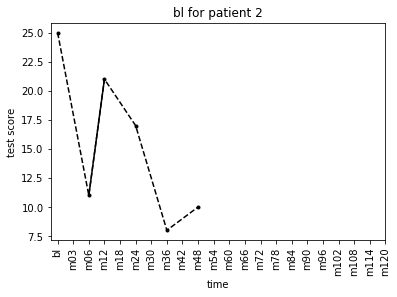
\includegraphics[width=0.5\textwidth]{images/cog_test.png}
        \end{center}
    \end{frame}

    \begin{frame}
        \frametitle{Cognitive Tests}
        \begin{center}
            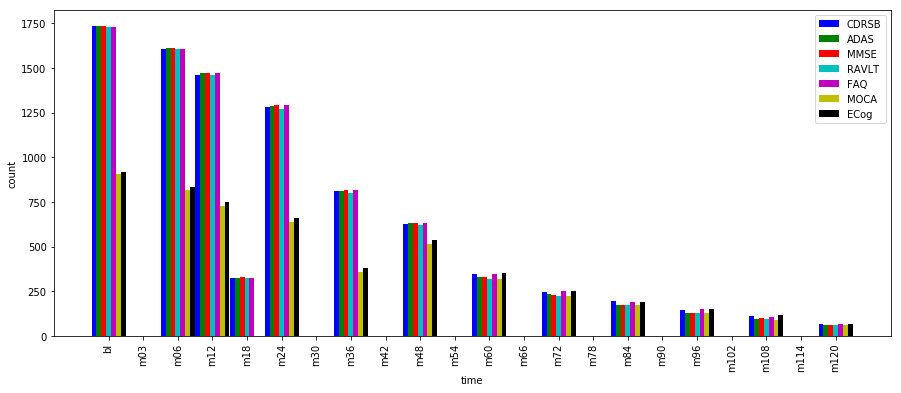
\includegraphics[width=\textwidth]{images/cog_times.png}
        \end{center}
    \end{frame}

    \begin{frame}
        \frametitle{CSF}
        Longitudinal \hfill 1255/1737 (72.3\%) \\
        \vspace{0.2in}
        Abnormal levels of certain proteins in the cerebrospinal fluid (CSF) are some of the earliest signs of Alzheimer's disease and can indicate abnormalities many years before symptom onset. \\
        \vspace{0.2in}
        This dataset contains amyloid-beta level, tau level, and phosphorylated tau level.
        \begin{center}
            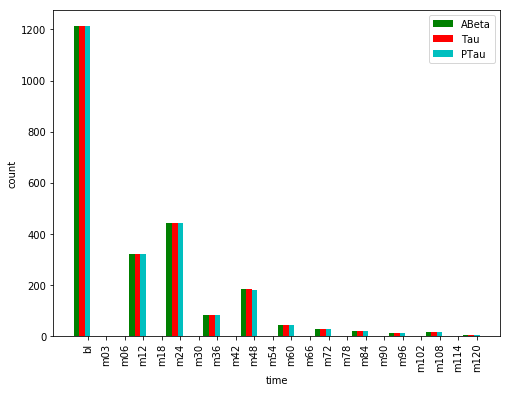
\includegraphics[height=0.4\paperheight]{images/csf_times.png}
            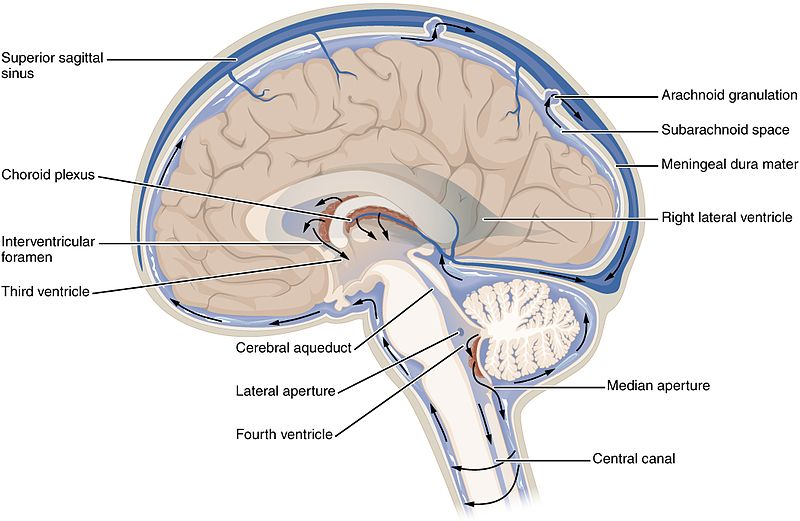
\includegraphics[height=0.4\paperheight]{images/csf.jpg}
        \end{center}
    \end{frame}

    \begin{frame}
        \frametitle{MRI}

        \begin{itemize}
            \item MRI \\
            TADPOLE datasets include three main types of structural MRI markers of atrophy: 1. ROI volumes 2. ROI cortical thicknesses 3. ROI surface areas
                \begin{itemize}
                    \item FreeSurfer (cross-sectional) \hfill 1735/1737 Patients (99.9\%)
                    \item FreeSurfer (longitudinal) \hfill 1105/1737 Patients (63.6\%)
                \end{itemize}
            \item Diffusion Tensor Imaging (DTI) \hfill 249/1737 Patients (14.3\%)\\
            DTI can measure the degeneration of white matter (connections between neurons) in the brain. This is done by analyzing the diffusion of water molecules along the neuron fibre connections.
        \end{itemize}
        \begin{center}
            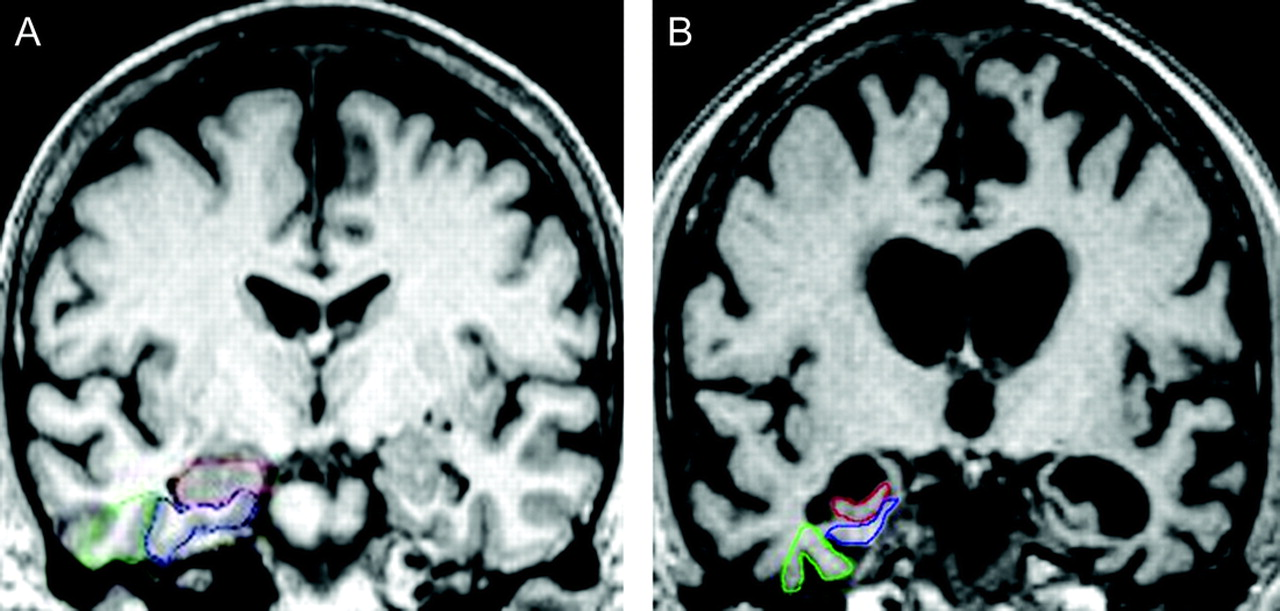
\includegraphics[height=0.22\paperheight]{images/mri_image.jpg}
            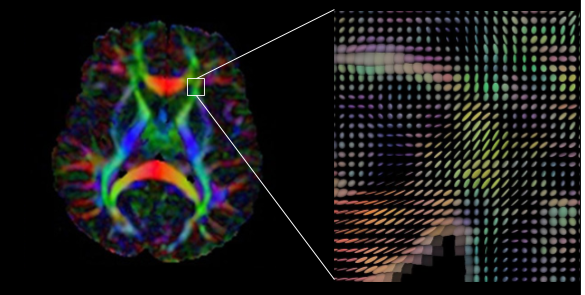
\includegraphics[height=0.22\paperheight]{images/dti.png}
        \end{center}
    \end{frame}

    \begin{frame}
        \frametitle{MRI}
        \begin{center}
            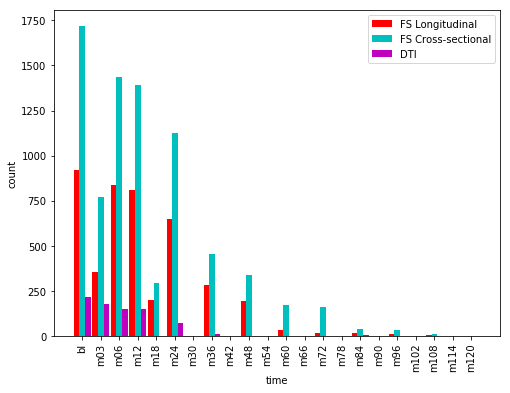
\includegraphics[width=0.75\textwidth]{images/mri_times.png}
        \end{center}
    \end{frame}

    \begin{frame}
        \frametitle{PET}
        \begin{itemize}
            \item FDG PET ROI Averages \hfill 1401/1737 Patients (80.7\%)\\
            measure cell metabolism, where cells affected by AD show reduced metabolism
            \item AV45 PET ROI averages \hfill 1094/1737 Patients (63.0\%) \\
            measures amyloid-beta load in the brain, where amyloid-beta is a protein that mis-folds (i.e. its 3D structure is not properly constructed), which then leads to AD
            \item AV1451 PET ROI \hfill 85/1737 Patients (4.9\%)\\
            measures tau load in the brain, where tau is another protein which, when abnormal, damages neurons and thus leads to AD
        \end{itemize}
        \begin{center}
            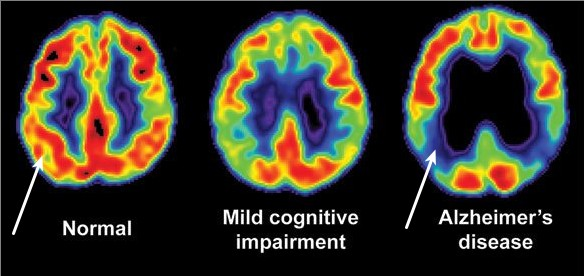
\includegraphics[height=0.25\paperheight]{images/pet_image.jpg}
        \end{center}
    \end{frame}

    \begin{frame}
        \frametitle{PET}
        \begin{center}
            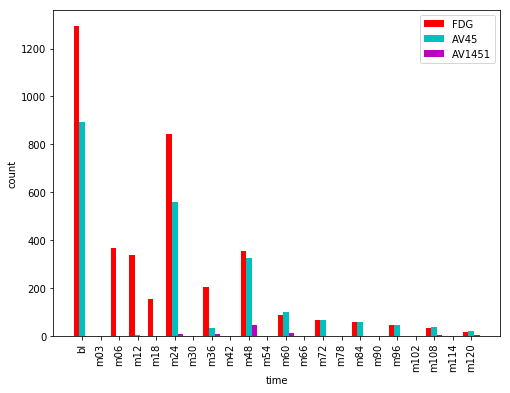
\includegraphics[width=0.75\textwidth]{images/pet_times.png}
        \end{center}
    \end{frame}

    \begin{frame}
        \frametitle{Brain Visualization}
        All brain imaging data, MRI, DTI, and PET, has been sectioned into regions of interest ROIs, and such can be visualized with the python nilearn package.\\
        \begin{center}
            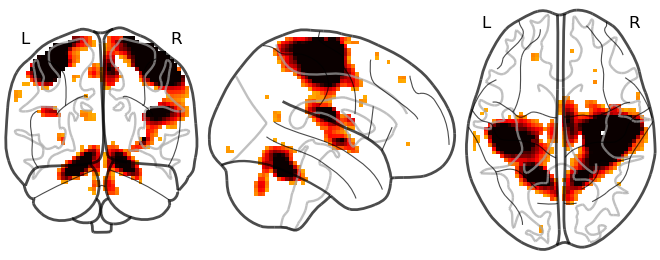
\includegraphics[width=0.9\textwidth]{images/glass_brain.png}
        \end{center}
    \end{frame}

    \begin{frame}
        \frametitle{Data Access}
        \begin{columns}
        \begin{column}{0.4\textwidth}
            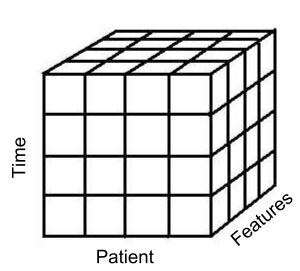
\includegraphics[width=\textwidth]{images/cube.png}
        \end{column}
        \begin{column}{0.6\textwidth}
            \begin{itemize}
                \item Linked on Slack
                \item Data and Name Files for all Modalities
                    \begin{itemize}
                        \item finished\_(modaility)\_dat.npy
                        \item (modaility)tags.npy
                    \end{itemize}
                \item Dimensions: (patient, time, features)
                \item Size: (1737 x 22 x feature length)
            \end{itemize}
        \end{column}
        \end{columns}
    \end{frame}

    \begin{frame}
        \frametitle{Links}
        \begin{itemize}
            \item \href{https://tadpole.grand-challenge.org/Data/}{TADPOLE Website Data Information}
            \item \href{https://arxiv.org/pdf/1805.03909.pdf}{TADPOLE Challenge Paper}
        \end{itemize}
    \end{frame}


    % Questions Slide
    \begin{frame}
        \begin{center}
        {\Huge \fontspec{Montserrat SemiBold} Questions}
        \end{center}
    \end{frame}


\end{document}
